\section{Abstract}
Die strongSwan Open Source VPN Software ist weltweit im Einsatz. Es besteht schon länger die Nachfrage nach einer grafischen Managementoberfläche, welche das Konfigurieren und Starten von IPsec Verbindungen erleichtert.\\
Zur Umsetzung dieses Problems stellt strongSwan das Versatile IKE Configuration Interface (VICI) zur Verfügung, welches für diverse Programmiersprachen eine JSON-artige Schnittstelle bietet. \\
Im Rahmen dieser Bachelorarbeit ist die Applikation strongMan entstanden, die auf dem Python Webframework Django basiert.\\

Der strongMan unterstützt eine benutzerfreundliche Konfiguration diverser Internet Key Exchange (IKEv2) Authentisierungsmethoden, welche in einer Datenbank persistiert werden. Diese können auf der Hauptübersicht bearbeitet werden. Weiter lassen sich diese Verbindungen auf- und abbauen. Das Starten hat zur Folge, dass der strongMan die Konfigurationsdaten in ein Dictionary umwandelt und dem strongSwan per Unix Socket über die VICI-Schnittstelle übergibt. Ist die Verbindung erfolgreich etabliert werden Statusinformationen zu Traffic Selectoren, sowie Datenin- und Output dargestellt. Parallel dazu werden die Logmessages des strongSwan ausgelesen und visualisiert.\\

\begin{wrapfigure}{r}{0.5\textwidth}
  \begin{center}
    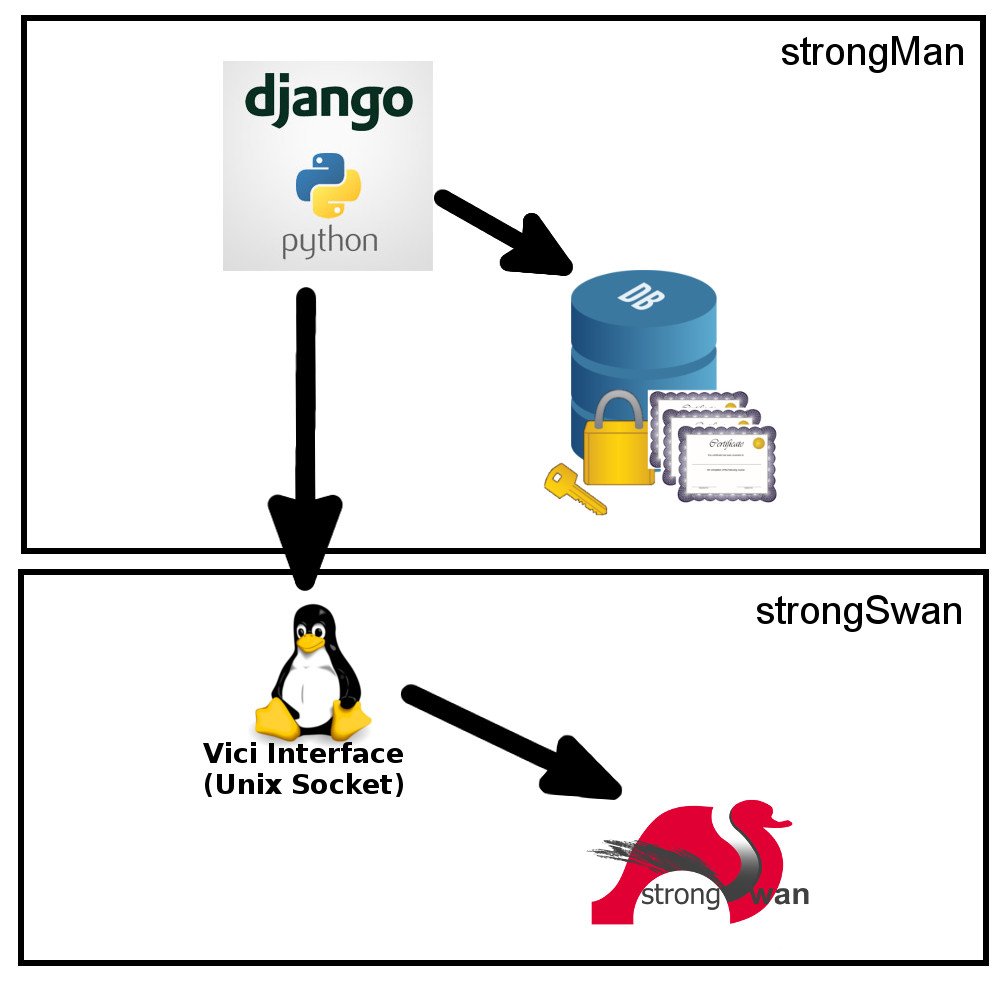
\includegraphics[width=230px]{images/strongman_ubersicht.jpg}
  \end{center}
    \caption[Übersicht]{Übersicht}
\end{wrapfigure}

Die interne Zertifikatsverwaltung ermöglicht den Upload von PKCS1, PKCS8, PKCS12 und X.509 Schlüsselkontainern. Diese werden in der Datenbank gespeichert, wobei alle sensitiven Daten verschlüsselt abgelegt werden. Nach dem Erfassen können wichtige Felder wie der Canonical Name (CNAME) direkt in der Zertifikatsvorschau eingesehen werden. Zusätzlich werden auch alle durch den strongSwan verwalteten Zertifikate in der strongMan Applikation dargestellt.\\

Zusätzlich bietet eine Informationsseite Übersicht über die verwendete strongSwan Version und allen installierten Plugins.\\


Der Fokus der strongMan Applikation zielt aktuell auf die Clientseite. In einem nächsten Schritt ist es möglich die Anwendung so zu erweitern, dass auch Serverfunktionalitäten hinzukommen. Dazu ist ein Administratormodus sinnvoll, der weitere Authentisierungsmethoden ermöglicht, die Konfigurationsmöglichkeiten ausbaut, zusätzliche Statusinformationen visualisiert und das Management von mehreren Security Associations (SA) implementiert. 
